\documentclass{article}


% if you need to pass options to natbib, use, e.g.:
%     \PassOptionsToPackage{numbers, compress}{natbib}
% before loading neurips_2023

% ready for submission
\usepackage[final]{neurips_2023}

% to avoid loading the natbib package, add option nonatbib:
%    \usepackage[nonatbib]{neurips_2023}


\usepackage[utf8]{inputenc} % allow utf-8 input
\usepackage[T1]{fontenc}    % use 8-bit T1 fonts
\usepackage{hyperref}       % hyperlinks
\usepackage{url}            % simple URL typesetting
\usepackage{booktabs}       % professional-quality tables
\usepackage{amsfonts}       % blackboard math symbols
\usepackage{nicefrac}       % compact symbols for 1/2, etc.
\usepackage{microtype}      % microtypography
\usepackage{xcolor}         % colors
\usepackage{graphicx}       % addtional package for show figures


\begin{document}


\maketitle


%%%%%%% Part 4 Text Features Start %%%%%%%%%

\section{Text Features}

\subsubsection{(a) Text‑embedding clustering}   % third‑level  
We load 35\,826 sentence‑transformer embeddings (1\,024 dims, unit‑norm).  
A PCA that retains 90\,\% variance compresses them to 100 dimensions;  
K‑Means is then swept over $k=5\dots20$.  
Figure~\ref{fig:text_silhouette} shows a local silhouette peak at 
\mbox{$k=15$} ($s=0.071$), so we adopt \textbf{$k=15$}.  
t‑SNE projections for $k=11$ and 15 (Figure~\ref{fig:text_tsne}) confirm that  
$k=15$ better separates colour islands while keeping clusters interpretable.

\begin{figure}[h]
  \centering
  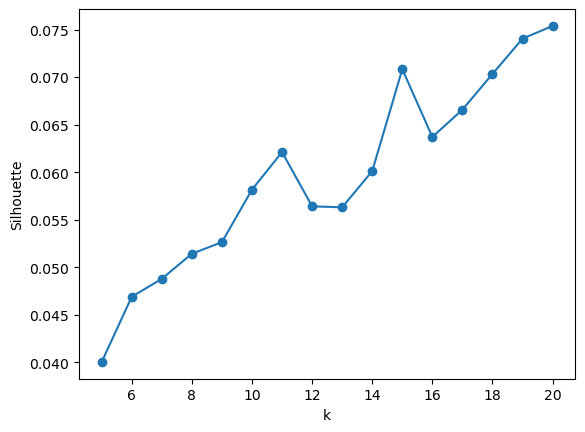
\includegraphics[width=.55\linewidth]{figs_tang/04_silhouette_k.png}
  \caption{Silhouette over $k=5\dots20$ (text embeddings).}
  \label{fig:text_silhouette}
\end{figure}

\begin{figure}[h]
  \centering
  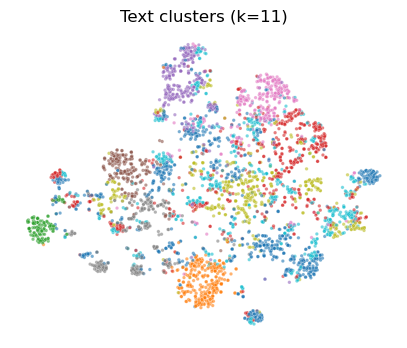
\includegraphics[width=.45\linewidth]{figs_tang/04_text_cluster11.png}\hfill
  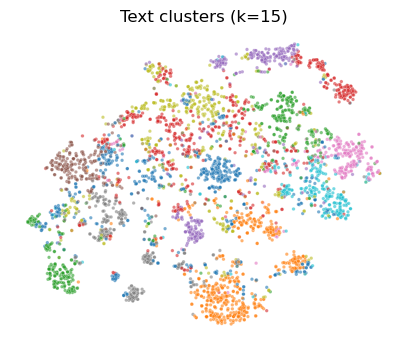
\includegraphics[width=.45\linewidth]{figs_tang/04_text_cluster15.png}
  \caption{t‑SNE colour‑map of text clusters for $k=11$ (left) and $k=15$ (right).}
  \label{fig:text_tsne}
\end{figure}

Listening to five random samples per cluster yields the themes in
Table~\ref{tab:text_themes}; they cover bells (\texttt{C0}), buzzing/sirens
(\texttt{C1}), dog‑/bird‑calls (\texttt{C2}), water/rain (\texttt{C3}) \emph{etc.},
validating the semantic coherence.

\begin{table}[h]
  \caption{Manual auditory label of the 15 text clusters.}
  \label{tab:text_themes}
  \centering
  \small
  \begin{tabular}{cl}
    \toprule
    Cluster & Dominant sound theme \\ \midrule
    0 & bell sound \\
    1 & buzzing sound / siren \\
    2 & dogs or birds \\
    3 & water / rain \\
    4 & repeating mechanical sound \\
    5 & vocal sound \\
    6 & engine / vehicle \\
    7 & high‑pitched vocal (kitten / child) \\
    8 & high‑pitched noise / drill \\
    9 & high‑level ambience \\
    10 & hissing / scratching \\
    11 & generic animal farm / birds \\
    12 & high‑pitched repeating motor \\
    13 & rhythmic footsteps / cheering \\
    14 & low‑level ambience / jazz \\
    \bottomrule
  \end{tabular}
\end{table}

\subsubsection{(b) Dog \& Cat labelling function}
A hybrid labelling function—regex dictionary
\texttt{\small(bark$\mid$woof$\mid$puppy), (meow$\mid$purr$\mid$kitten)} plus
cosine\,>\,0.35 to class prototypes—identifies \textbf{1\,483 dog} and
\textbf{731 cat} annotations.  
Entropy over the 15 clusters is 0.073 (dog) / 0.073 (cat), i.e.\ $>$80\,\% of
each class falls into only two clusters.
Figure~\ref{fig:dogcat_tsne} visualises the tight grouping in t‑SNE space.

\begin{figure}[h]
  \centering
  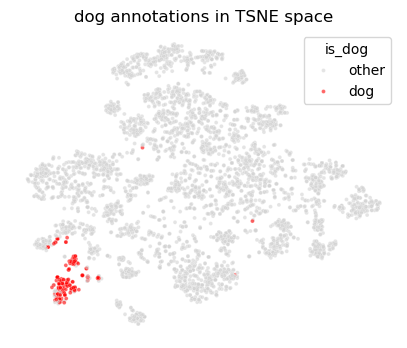
\includegraphics[width=.42\linewidth]{figs_tang/04_dog_annotations_in_tsne_space.png}\hfill
  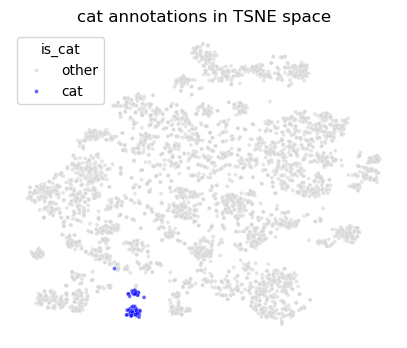
\includegraphics[width=.42\linewidth]{figs_tang/04_cat_annotations_in_tsne_space.png}
  \caption{Dog (left) and cat (right) annotations highlighted in t‑SNE space.}
  \label{fig:dogcat_tsne}
\end{figure}

\subsubsection{(c) Alignment between text and audio clusters}
The 51\,966 audio region vectors were clustered with $k=4$
(cf.\ Section~3c).  
After aligning on \texttt{(filename, onset, offset)} rounded to 1\,ms,
35\,552 event pairs remain; four extremely small text clusters ($<0.3\%$
each, duration $<$1 frame) have no audio match and appear as zero rows.
The cross‑tab in Figure~\ref{fig:text_audio_heat} shows clear correspondences
(bells $\rightarrow$ audio 0, speech $\rightarrow$ 1, animals $\rightarrow$ 2,
water/ambience $\rightarrow$ 3).  
Normalised Mutual Information between the 15 text clusters and the 4 audio
clusters is \textbf{NMI = 0.28}.

\begin{figure}[h]
  \centering
  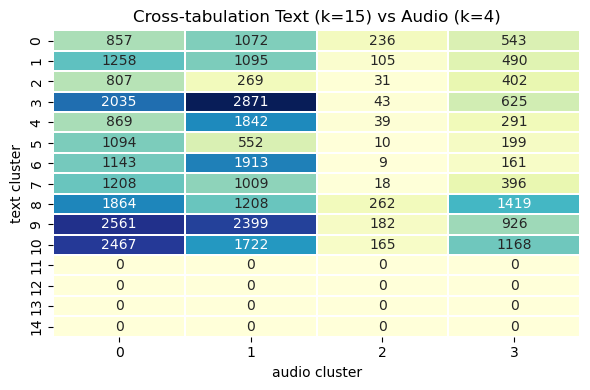
\includegraphics[width=.7\linewidth]{figs_tang/04_text_audio_heatmap_k15.png}
  \caption{Cross‑tabulation of text clusters ($k=15$) vs.\ audio clusters
           ($k=4$). Rows 11–14 are empty because those text clusters
           contain only sub‑frame annotations without audio features.}
  \label{fig:text_audio_heat}
\end{figure}

\paragraph{Take‑aways.}
Text embeddings cluster into 15 semantically coherent groups; the dog/cat
labelling function verifies tight intracluster cohesion.  
Cross‑modal NMI 0.28 indicates a moderate but meaningful alignment between
text and audio spaces, sufficient to transfer weak labels across modalities.

%%%%%%% Part 4 Text Features Finish %%%%%%%%%

\end{document}